\documentclass[12pt, a4paper]{ctexart}
\usepackage{geometry}
\geometry{left=2.5cm, right=2.5cm, top=3cm, bottom=3cm}
\usepackage{graphicx}
\usepackage{xcolor}
\usepackage{circuitikz}
\usepackage{subcaption}
\usepackage{float}
\usepackage{amsmath}
\usepackage{listings}
\usetikzlibrary{arrows, shapes.gates.logic.US, positioning}
\ctikzset{
    logic ports=ieee,
    logic ports/scale=0.8,
    multipoles/flipflop/pin spacing=0.4
}
\lstset{
    basicstyle=\ttfamily\small,
    frame=single,
    framesep=5pt,
    xleftmargin=10pt,
    xrightmargin=10pt,
    keywordstyle=\color{blue},
    commentstyle=\color{gray},
    breaklines=true
}

\begin{document}

% 封面
\begin{titlepage}
    \centering
    \vspace*{5cm}
    {\Huge\bfseries 实验报告\par}
    \vspace{2cm}
    {\Large 课程：数字逻辑与计算机组成\par}
    \vspace{1cm}
    {\Large 实验五：存储器及数据通路设计\par}
    \vspace{4cm}
    {\large 姓名：\underline{\makebox[4cm]{郑袭明}}\par}
    \vspace{1cm}
    {\large 学号：\underline{\makebox[4cm]{251502027}}\par}
    \vspace{1cm}
    {\large 日期：\today\par}
\end{titlepage}

\tableofcontents
\enlargethispage{\baselineskip}
\newpage

\section{实验目的}

\begin{enumerate}
    \item 掌握利用 ROM 组件实现指令存储器的设计方法。
    \item 掌握 ASCII 点阵字库的使用方法。
    \item 掌握利用 RAM 组件实现按字节存取的数据存储器的设计方法。
    \item 掌握实现 RV32I 存取指令的设计方法。
    \item 掌握 RV32I 下地址逻辑部件的设计方法
    \item 掌握 RV32I 指令译码、反汇编的实现方法
    \item 掌握 RV32I 立即数扩展器的设计方式
    \item 根据 RV32I 指令执行过程，掌握 RV32I 运算类指令数据通路的设计方法
    \item 掌握跳转控制器的设计方法
\end{enumerate}

\section{实验一：只读存储器实验}

\subsection{整体方案设计}

根据输入的 ASCII 码，从 ROM 中读取字符点阵数据，然后在 LED 点阵组件上显示。

\begin{table}[H]
    \centering
    \begin{tabular}{|c|c|}
        \hline
        引脚 & 功能 \\
        \hline
        Code[6:0] & ASCII 码输入 \\
        row1-16[7:0] & 字符点阵数据输出 \\
        CodeErr & ASCII 码错误指示 \\
        \hline
    \end{tabular}
    \caption{只读存储器实验引脚功能表}
\end{table}

\subsection{电路设计}

\begin{figure}[H]
    \centering
    \begin{circuitikz}
        \node[
            muxdemux,
            muxdemux def={Lh=2, Rh=2, w=2, NR=1, NL=2, NB=1, NT=1},
            muxdemux label={T1=bin, B1=bout}
        ] (sub) at (0,0) {Sub};
        \node[left] (code) at (sub.lpin 1) {Code};
        \node[left] at (sub.lpin 2) {\texttt{0x20}};
        \node[below] (err) at (sub.bpin 1) {CodeErr};
        \node[
            muxdemux,
            muxdemux def={Lh=3, Rh=3, w=6, NL=1, NR=1, NT=0, NB=1},
            muxdemux label={L1=A, R1=D, B1=sel},
            anchor=lpin 1
        ] (rom) at (sub.rpin 1) {ROM};
        \node[below] at (rom.bpin 1) {$\sim$CodeErr};
        \node[right] at (rom.rpin 1) {rows};
    \end{circuitikz}
    \caption{只读存储器实验原理图}
\end{figure}

\begin{figure}[H]
    \centering
    
\includegraphics[width=\textwidth]{assets/exp1/circuit.png}
    \caption{只读存储器实验电路图}
\end{figure}

\subsection{仿真结果}

\begin{figure}[H]
    \centering
    
\includegraphics[width=\textwidth]{assets/exp1/sim1.png}
    
\includegraphics[width=\textwidth]{assets/exp1/sim2.png}
    \caption{只读存储器实验仿真结果(a)}
\end{figure}

\begin{figure}[H]
    \centering
    
\includegraphics[width=\textwidth]{assets/exp1/sim3.png}
    
\includegraphics[width=\textwidth]{assets/exp1/sim4.png}
    \caption{只读存储器实验仿真结果(b)}
\end{figure}

\begin{table}[H]
    \centering
    \begin{tabular}{|c|c|c|}
        \hline
        Code & rows & CodeErr \\
        \hline
        < 0x20 & 0xxx & 1 \\
        $\geq$ 0x20 & 0x00-0xFF & 0 \\
        \hline
    \end{tabular}
    \caption{只读存储器实验真值表}
\end{table}

\subsection{错误现象及分析}

在完成实验的过程中，没有遇到任何错误。

\section{实验二：数据存储器实验}

\subsection{整体方案设计}

\begin{lstlisting}[language=Verilog, caption={数据存储器实验设计原理}]
module dmem (
    input [31:0] Addr,
    output reg [31:0] Dout,
    input [31:0] Din,
    input clk,
    input [2:0] MemOp,
    input WE
);

  reg [31:0] mem[0:1023];
  wire [9:0] word_addr = Addr[11:2];
  wire [1:0] byte_offset = Addr[1:0];
  wire [31:0] data = mem[word_addr];

  always @(posedge clk) begin
    case (MemOp)
      3'b000: begin
        case (byte_offset)
          2'b00:   Dout <= {{24{data[7]}}, data[7:0]};
          2'b01:   Dout <= {{24{data[15]}}, data[15:8]};
          2'b10:   Dout <= {{24{data[23]}}, data[23:16]};
          2'b11:   Dout <= {{24{data[31]}}, data[31:24]};
        endcase
      end
      3'b001: begin
        case (byte_offset)
          2'b00:   Dout <= {{16{data[15]}}, data[15:0]};
          2'b10:   Dout <= {{16{data[31]}}, data[31:16]};
          default: Dout <= 32'b0;
        endcase
      end
      3'b010:  Dout <= data;
      3'b100: begin
        case (byte_offset)
          2'b00:   Dout <= {24'b0, data[7:0]};
          2'b01:   Dout <= {24'b0, data[15:8]};
          2'b10:   Dout <= {24'b0, data[23:16]};
          2'b11:   Dout <= {24'b0, data[31:24]};
        endcase
      end
      3'b101: begin
        case (byte_offset)
          2'b00:   Dout <= {16'b0, data[15:0]};
          2'b10:   Dout <= {16'b0, data[31:16]};
          default: Dout <= 32'b0;
        endcase
      end
      default: Dout <= 32'b0;
    endcase
  end

  always @(posedge clk) begin
    if (WE) begin
      case (MemOp)
        3'b000: begin
          case (byte_offset)
            2'b00:   mem[word_addr] = {data[31:8], Din[7:0]};
            2'b01:   mem[word_addr] = {data[31:16], Din[7:0], data[7:0]};
            2'b10:   mem[word_addr] = {data[31:24], Din[7:0], data[15:0]};
            2'b11:   mem[word_addr] = {Din[7:0], data[23:0]};
          endcase
        end
        3'b001: begin
          case (byte_offset)
            2'b00:   mem[word_addr] = {data[31:16], Din[15:0]};
            2'b10:   mem[word_addr] = {Din[15:0], data[15:0]};
            default: mem[word_addr] = 32'b0;
          endcase
        end
        3'b010:  mem[word_addr] <= Din;
        default: mem[word_addr] <= 32'b0;
      endcase
    end
  end

endmodule
\end{lstlisting}

\begin{table}[H]
    \centering
    \begin{tabular}{|c|c|}
        \hline
        引脚 & 功能 \\
        \hline
        Addr[31:0] & 地址输入 \\
        Dout[31:0] & 数据输出 \\
        Din[31:0] & 数据输入 \\
        clk & 时钟信号 \\
        MemOp[2:0] & 存储器操作类型 \\
        WE & 写使能信号 \\
        CLR & 存储器清零信号 \\
        AlignErr & 地址对齐错误指示 \\
        \hline
    \end{tabular}
    \caption{数据存储器实验引脚功能表}
\end{table}

\subsection{电路设计}

\begin{figure}[H]
    \centering
    
\includegraphics[width=\textwidth]{assets/exp2/circuit.png}
    \caption{数据存储器实验电路图}
\end{figure}

电路图中的自定义元件为输入全部反相的三输入异或门（当且仅当一个输入为高电平输出高电平），
功能是当且仅当两个输入为高电平输出高电平。

\begin{figure}[H]
    \centering
    \begin{circuitikz}
        \node[
            muxdemux,
            muxdemux def={Lh=3, Rh=3, w=4, NL=2, NR=1, NT=0, NB=1}
        ] (decd) at (0,0) {};
        \node[left] at (decd.lpin 1) {Addr};
        \node[left] at (decd.lpin 2) {MemOp};
        \node[below] at (decd.bpin 1) {AlignErr};
        \node[right] at (decd.rpin 1) {SEL[3:0]};
        \node[
            muxdemux,
            muxdemux def={Lh=3, Rh=3, w=6, NL=2, NR=1, NT=0, NB=4},
            muxdemux label={L1=A, L2=D, R1=D, B1=str, B2=sel, cB3=1, B4=clr}
        ] (ram) at (7.5,0) {RAM$\times$4};
        \node[left] at (ram.lpin 1) {Addr};
        \node[left] at (ram.lpin 2) {Din (Mux)};
        \node[below] at (ram.bpin 1) {WE};
        \node[below] at (ram.bpin 2) {SEL};
        \node[below] at (ram.bpin 3) {CLK};
        \node[below] at (ram.bpin 4) {CLR};
        \node[right] at (ram.rpin 1) {Dout (Mux)};
    \end{circuitikz}
    \caption{数据存储器实验原理图}
\end{figure}

\subsection{仿真结果}

\begin{figure}[H]
    \centering
    
\includegraphics[width=0.9\textwidth]{assets/exp2/sim1.png}
    
\includegraphics[width=0.9\textwidth]{assets/exp2/sim2.png}
    
\includegraphics[width=0.9\textwidth]{assets/exp2/sim3.png}
    \caption{数据存储器实验仿真结果(a)}
\end{figure}

\begin{figure}[H]
    \centering
    
\includegraphics[width=0.9\textwidth]{assets/exp2/sim4.png}
    \caption{数据存储器实验仿真结果(b)}
\end{figure}

\begin{table}[H]
    \centering
    \begin{tabular}{|c|c|c|}
        \hline
        MemOp & Addr[1:0] & 结果 \\
        \hline
        000 & 00 & Dout = {{24{data[7]}}, data[7:0]} \\
        000 & 01 & Dout = {{24{data[15]}}, data[15:8]} \\
        000 & 10 & Dout = {{24{data[23]}}, data[23:16]} \\
        000 & 11 & Dout = {{24{data[31]}}, data[31:24]} \\
        001 & 00 & Dout = {{16{data[15]}}, data[15:0]} \\
        001 & 10 & Dout = {{16{data[31]}}, data[31:16]} \\
        010 & xx & Dout = data \\
        100 & 00 & Dout = {24'b0, data[7:0]} \\
        100 & 01 & Dout = {24'b0, data[15:8]} \\
        100 & 10 & Dout = {24'b0, data[23:16]} \\
        100 & 11 & Dout = {24'b0, data[31:24]} \\
        101 & 00 & Dout = {16'b0, data[15:0]} \\
        101 & 10 & Dout = {16'b0, data[31:16]} \\
        \hline
    \end{tabular}
    \caption{数据存储器实验真值表}
\end{table}

\subsection{错误现象及分析}

\subsubsection*{三输入异或门行为错误}

Logisim 实验推荐版本为 2.16.1.3，而评测机的版本为 2.15.0.2 (华中科技大学修改版，
课程中没有提供该版本的文件，无法通过正常手段获取)，
前者的三输入异或门默认行为是“当且仅当一个输入为高电平输出高电平”，
而后者的三输入异或门默认行为是“当有奇数个输入为高电平输出高电平”。

翻阅源码可知，Logisim 不会在文件中储存对应默认行为的设置，也就是说，
“当且仅当一个输入为高电平输出高电平”不会被课程提供版本的 Logisim 储存，
那么这个行为也就不可能在评测机上出现了，除非获取到评测机的版本，然后在该版本下修改文件。

而在实验中我正好需要“当且仅当一个输入为高电平输出高电平”的行为，
所以本地和在线测试都完全正常，而评测时始终不通过。

最终我使用了一个自定义元件来模拟该三输入异或门的行为，结果正常。

\subsubsection*{自定义元件方向错误}

Logisim 中的自定义元件默认方向和储存方向不同，导致在电路图中放置时会显示正确而保存错误，
解决方法是重启 Logisim 后调整方向，重新保存一次。

\subsubsection*{总结}

Logisim-Ita 长时间没有更新，评测机上的版本更是搞笑；
堂堂南京大学的课程居然用华中科技大学的修改版，还有不少适配问题。

望课程尽快更改 Logisim 版本，望后来者不要重蹈覆辙。

\section{实验三：取指令部件实验}

\subsection{整体方案设计}

使用加法器来进行计算下一条指令的地址，存入 PC 寄存器中，并从 ROM 中取出指令。

\begin{table}[H]
    \centering
    \begin{tabular}{|c|c|}
        \hline
        引脚 & 功能 \\
        \hline
        PC[31:0] & 程序计数器输出 \\
        IR[31:0] & 指令输出 \\
        Init Addr & 程序计数器初始值输入 \\
        BusA [31:0] & 加法器输入A \\
        Imm[31:0] & 加法器输入B \\
        CLK & 时钟信号 \\
        Reset & 复位信号 \\
        NPCASrc & 加法器输入A选择信号 \\
        NPCBSrc & 加法器输入B选择信号 \\
        \hline
    \end{tabular}
    \caption{取指令部件实验引脚功能表}
\end{table}

\subsection{电路设计}

\begin{figure}[H]
    \centering
    \begin{circuitikz}
        \node[
            muxdemux,
            muxdemux def={Lh=2, Rh=2, w=2, NR=1, NL=2, NB=1, NT=1},
            muxdemux label={T1=cin, B1=cout}
        ] (add) at (0,0) {Add};
        \node[left] at (add.lpin 1) {NPCASrc ? BusA : PC};
        \node[left] at (add.lpin 2) {NPCBSrc ? Imm : 0x4};
        \node[
            muxdemux,
            muxdemux def={Lh=2, Rh=1, w=1.5, NR=1, NL=2, NB=1, NT=0},
            muxdemux label={L1=0, L2=1},
            anchor=lpin 1
        ] (mux) at (add.rpin 1) {};
        \draw (mux.lpin 2) -- ++(0,-1) node[below] {Init Addr};
        \node[below] at (mux.bpin 1) {reset};
        \node[
            muxdemux,
            muxdemux def={Lh=2, Rh=2, w=1.5, NL=1, NR=1, NB=1, NT=0},
            muxdemux label={cB1=1},
            anchor=lpin 1
        ] (reg) at (mux.rpin 1) {Reg};
        \node[below] at (reg.bpin 1) {clk};
        \draw (reg.rpin 1) -- ++(0,-1) node[below] {PC};
        \node[
            muxdemux,
            muxdemux def={Lh=3, Rh=3, w=6, NL=1, NR=1, NT=0, NB=1},
            muxdemux label={L1=A, R1=D, B1=sel},
            anchor=lpin 1
        ] (rom) at (reg.rpin 1) {ROM};
        \node[right] at (rom.rpin 1) {IR};
    \end{circuitikz}
    \caption{取指令部件实验原理图}
\end{figure}

\begin{figure}[H]
    \centering
    
\includegraphics[width=\textwidth]{assets/exp3/circuit.png}
    \caption{取指令部件实验电路图}
\end{figure}

\subsection{仿真结果}

\begin{figure}[H]
    \centering
    
\includegraphics[width=\textwidth]{assets/exp3/sim1.png}
    \caption{取指令部件实验仿真结果(a)}
\end{figure}

\begin{figure}[H]
    \centering
    
\includegraphics[width=\textwidth]{assets/exp3/sim2.png}
    
\includegraphics[width=\textwidth]{assets/exp3/sim3.png}
    
\includegraphics[width=\textwidth]{assets/exp3/sim4.png}
    \caption{取指令部件实验仿真结果(b)}
\end{figure}

\begin{table}[H]
    \centering
    \begin{tabular}{|c|c|c|}
        \hline
        NPCASrc & NPCBSrc & NextPC \\
        \hline
        0 & 0 & PC + 4 \\
        0 & 1 & PC + Imm \\
        1 & 1 & BusA + Imm \\
        \hline
    \end{tabular}
    \caption{取指令部件实验真值表}
\end{table}

\subsection{错误现象及分析}

在完成实验的过程中，没有遇到任何错误。

\section{实验四：取操作数部件实验}

\subsection{整体方案设计}

\begin{figure}[H]
    \centering
    \begin{tikzpicture}[>=stealth]
        \node (IR) {IR};
        \node[draw, left=of IR] (ext) {立即数拓展器};
        \node[draw, right=of IR] (reg) {寄存器堆};
        \node[left=of ext] (imm) {imm};
        \draw[->] (IR) -- (ext);
        \draw[->] (ext) -- (imm);
        \draw[->] (IR) -- (reg);
        \node[below=of ext] (extop) {ExtOp};
        \draw[->] (extop) -- (ext);
        \node[below=of reg] (regwr) {RegWr};
        \node[right=of reg] (bus) {BusA, BusB};
        \draw[->] (regwr) -- (reg);
        \draw[->] (reg) -- (bus);
    \end{tikzpicture}
    \caption{取操作数部件实验整体方案设计}
\end{figure}

\begin{table}[H]
    \centering
    \begin{tabular}{|c|c|c|c|}
        \hline
        引脚 & 功能 & 引脚 & 功能 \\
        \hline
        IR[31:0] & 指令输入 & Imm[31:0] & 立即数输出 \\
        BusW[31:0] & 寄存器堆写回数据输入 & BusA[31:0] & 寄存器堆输出A \\
        PC[31:0] & 程序计数器输入 & BusB[31:0] & 寄存器堆输出B \\
        ExtOp[1:0] & 立即数拓展类型选择信号 & DataA[31:0] & ALU 输入A \\
        RegWr & 寄存器写使能信号 & DataB[31:0] & ALU 输入B \\
        ALUASrc & ALU 输入A选择信号 & OpCode[6:0] & 指令操作码 \\
        ALUBSrc[1:0] & ALU 输入B选择信号 & Func3[2:0] & 指令 funct3 字段 \\
        clk & 时钟信号 & Func7[6:0] & 指令 funct7 字段 \\
        \hline
    \end{tabular}
    \caption{取操作数部件实验引脚功能表}
\end{table}

\subsection{电路设计}

\begin{figure}[H]
    \centering
    \begin{circuitikz}
        \node[
            muxdemux,
            muxdemux def={Lh=3, Rh=3, w=3, NL=1, NR=1, NT=0, NB=1},
            muxdemux label={L1=Instr, B1=Extop, R1=Imm}
        ] (ext) at (0,0) {};
        \node[left] at (ext.lpin 1) {IR};
        \node[below] at (ext.bpin 1) {ExtOp};
        \node[right] at (ext.rpin 1) {Imm};
        \node[
            muxdemux,
            muxdemux def={Lh=5, Rh=5, w=5, NL=4, NR=2, NB=1, NT=1},
            muxdemux label={
                L1=R1\#, L2=R2\#, L3=W\#, L4=Din,
                R1=R1, R2=R2, T1=WE, cB1=1
            }
        ] (reg) at (6,0) {Reg};
        \node[left] at (reg.lpin 1) {IR[19:15]};
        \node[left] at (reg.lpin 2) {IR[24:20]};
        \node[left] at (reg.lpin 3) {IR[11:7]};
        \node[left] at (reg.lpin 4) {BusW};
        \node[below] at (reg.bpin 1) {clk};
        \node[above] at (reg.tpin 1) {RegWr};
        \node[right] at (reg.rpin 1) {BusA};
        \node[right] at (reg.rpin 2) {BusB};
    \end{circuitikz}
    \caption{取操作数部件实验原理图}
\end{figure}

其中

\begin{itemize}
    \item \texttt{OpCode = IR[6:0]}
    \item \texttt{Func3 = IR[14:12]}
    \item \texttt{Func7 = IR[31:25]}
    \item \texttt{DataA = (ALUASrc == 0) ? BusA : PC}
    \item \texttt{DataB = (ALUBSrc == 00) ? BusB : (ALUBSrc == 01) ? 4 : Imm}
\end{itemize}

\begin{figure}[H]
    \centering
    \subcaptionbox{IDU}{
\includegraphics[width=0.6\textwidth]{assets/exp4/circuit1.png}}
    \subcaptionbox{立即数拓展器}{
\includegraphics[width=0.3\textwidth]{assets/exp4/circuit2.png}}
    \caption{取操作数部件实验电路图}
\end{figure}

\subsection{仿真结果}

\begin{figure}[H]
    \centering
    
\includegraphics[width=\textwidth]{assets/exp4/sim1.png}
    
\includegraphics[width=\textwidth]{assets/exp4/sim2.png}
    \caption{取操作数部件实验仿真结果}
\end{figure}

\begin{table}[H]
    \centering
    \begin{tabular}{|c|c|c|}
        \hline
        ExtOp & Type & Imm \\
        \hline
        000 & immI & \{20\{Instr[31]\}, Instr[31:20]\} \\
        001 & immU & \{Instr[31:12], 12'b0\} \\
        010 & immS & \{20\{Instr[31]\}, Instr[31:25], Instr[11:7]\} \\
        011 & immB & \{19\{Instr[31]\},Instr[31], Instr[7], Instr[30:25], Instr[11:8], 1'b0\} \\
        100 & immJ & \{11\{Instr[31]\}, Instr[31], Instr[19:12], Instr[20], Instr[30:21], 1'b0\} \\
        \hline
    \end{tabular}
    \caption{取操作数部件实验真值表}
\end{table}

\subsection{错误现象及分析}

在完成实验的过程中，没有遇到任何错误。

\section{实验五：数据通路实验}

\subsection{整体方案设计}

\begin{figure}[H]
    \centering
    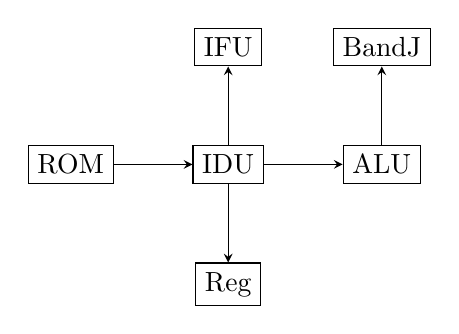
\begin{tikzpicture}[>=stealth]
        \node[draw] (idu) {IDU};
        \node[draw, below=of idu] (reg) {Reg};
        \node[draw, right=of idu] (alu) {ALU};
        \node[draw, above=of alu] (bandj) {BandJ};
        \node[draw, left=of idu] (rom) {ROM};
        \node[draw, above=of idu] (ifu) {IFU};
        \draw[->] (rom) -- (idu);
        \draw[->] (idu) -- (reg);
        \draw[->] (idu) -- (ifu);
        \draw[->] (idu) -- (alu);
        \draw[->] (alu) -- (bandj);
    \end{tikzpicture}
    \caption{数据通路实验整体方案设计}
\end{figure}

\begin{table}[H]
    \centering
    \begin{tabular}{|c|c|c|c|}
        \hline
        引脚 & 功能 & 引脚 & 功能 \\
        \hline
        Init Addr & 初始程序计数器地址 & ALUASrc & ALU第一个操作数来源选择 \\
        clk & 时钟输入 & ALUBSrc & ALU第二个操作数来源选择 \\
        ExtOp & 立即数扩展符号控制 & ALUctr & ALU操作控制信号 \\
        RegWr & 寄存器写使能 & PC & 当前程序计数器值输出 \\
        MemWr & 数据存储器写使能 & BusW & 总线写数据/写使能 \\
        MemtoReg & 写回数据来源 & Din & 数据输入 \\
        reset & 异步复位信号 & NPCASrc & 下一PC计算来源A选择 \\
        MemOp & 存储器操作类型 & NPCBSrc & 下一PC计算来源B选择 \\
        BandJ & 分支与跳转信号 &  &  \\
        \hline
    \end{tabular}
    \caption{数据通路实验引脚功能表}
\end{table}

\subsection{电路设计}

\begin{figure}[H]
    \centering
    
\includegraphics[width=0.9\textwidth]{assets/exp5/sch.png}
    \caption{数据通路实验原理图}
\end{figure}

\begin{figure}[H]
    \centering
    \subcaptionbox{数据通路}{
\includegraphics[width=0.6\textwidth]{assets/exp5/circuit1.png}}
    \subcaptionbox{BandJ}{
\includegraphics[width=0.3\textwidth]{assets/exp5/circuit2.png}}
    \caption{数据通路实验电路图}
\end{figure}

\subsection{仿真结果}

\begin{figure}[H]
    \centering
    
\includegraphics[width=\textwidth]{assets/exp5/sim1.png}
    
\includegraphics[width=\textwidth]{assets/exp5/sim2.png}
    
\includegraphics[width=\textwidth]{assets/exp5/sim3.png}
    \caption{数据通路实验仿真结果}
\end{figure}

\begin{table}[H]
    \centering
    \begin{tabular}{|c|c|c|}
        \hline
        序号 & 指令 & 控制信号赋值 \\ \hline
        1 & 008000ef & ExtOp=4, RegWr=1, ALUASrc=1, ALUBSrc=1, BandJ=1 \\ \hline
        2 & ffdff06f & ExtOp=4, RegWr=1, ALUASrc=1, ALUBSrc=1, BandJ=1 \\ \hline
        3 & 00100013 & RegWr=1, ALUBSrc=2 \\ \hline
        4 & deadc2b7 & ExtOp=1, RegWr=1, ALUBSrc=2, ALUctr=15 \\ \hline
        5 & eef28293 & RegWr=1, ALUBSrc=2 \\ \hline
        6 & 00c10337 & ExtOp=1, RegWr=1, ALUBSrc=2, ALUctr=15 \\ \hline
        7 & fee30313 & RegWr=1, ALUBSrc=2 \\ \hline
        8 & 0062be33 & RegWr=1, ALUctr=3 \\ \hline
        9 & 0062aeb3 & RegWr=1, ALUctr=2 \\ \hline
        10 & 01000513 & RegWr=1, ALUBSrc=2 \\ \hline
        11 & 00552023 & ExtOp=2, MemWr=1, ALUBSrc=2 \\ \hline
        12 & 00652223 & ExtOp=2, MemWr=1, ALUBSrc=2 \\ \hline
        13 & 00452f03 & RegWr=1, ALUBSrc=2, MemtoReg=1 \\ \hline
        14 & 00550f83 & RegWr=1, ALUBSrc=2, MemOp=5, MemtoReg=1 \\ \hline
        15 & 00654583 & RegWr=1, ALUBSrc=2, MemOp=1, MemtoReg=1 \\ \hline
        16 & 01f2f633 & RegWr=1, ALUctr=7 \\ \hline
        17 & 4102d693 & RegWr=1, ALUBSrc=2, ALUctr=13 \\ \hline
        18 & 01031713 & RegWr=1, ALUBSrc=2, ALUctr=1 \\ \hline
        19 & fdde00e3 & ExtOp=3, ALUctr=2, BandJ=4 \\ \hline
        20 & 00000073 &  \\ \hline
    \end{tabular}
    \caption{数据通路实验真值表}
\end{table}

\begin{table}[H]
    \centering
    \begin{tabular}{|c|c|c|c|}
        \hline
        序号 & 指令 & 指令解析 & 输出信号值 \\ \hline
        1 & 008000ef & Imm= 0x00000008 & NPCASrc=0, NPCBSrc=1 \\ \hline
        2 & ffdff06f & Imm= 0xfffffffc & NPCASrc=0, NPCBSrc=1 \\ \hline
        3 & 00100013 & 汇编语句：addi x0, x0, 1 & Busw= 0x00000001 \\ \hline
        4 & deadc2b7 & Imm= 0xdeadc & Busw= 0xdeadc000 \\ \hline
        5 & eef28293 & Imm= 0xfffffeef & Busw= 0xdeadbeef \\ \hline
        6 & 00c10337 & 汇编语句：lui x6, 0xc10 & Busw= 0x00c10000 \\ \hline
        7 & fee30313 & Imm= 0xffffffee & Busw= 0x00c0ffee \\ \hline
        8 & 0062be33 & 汇编语句：sltu x28, x5, x6 & Busw= 0x00000000 \\ \hline
        9 & 0062aeb3 & Rs1: x5, rs2: x6 & Busw= 0x00000001 \\ \hline
        10 & 01000513 & Imm= 0x00000010 & Busw= 0x00000010 \\ \hline
        11 & 00552023 & Imm= 0x00000000 & Din= 0xdeadbeef \\ \hline
        12 & 00652223 & 汇编语句：sw x6, 4(x10) & Din= 0x00c0ffee \\ \hline
        13 & 00452f03 & 汇编语句：lw x30, 4(x10) & Busw= 0x00c0ffee \\ \hline
        14 & 00550f83 & 汇编语句：lb x31, 5(x10) & Busw= 0xffffffff \\ \hline
        15 & 00654583 & Rd: x11 & Busw= 0x000000c0 \\ \hline
        16 & 01f2f633 & Rd: x12 & Busw= 0xdeadbeef \\ \hline
        17 & 4102d693 & Imm= 0x00000410 & Busw= 0xffffdead \\ \hline
        18 & 01031713 & Imm= 0x00000010 & Busw= 0xffee0000 \\ \hline
        19 & fdde00e3 & Imm= 0xffffffc0 & NPCASrc= 0, NPCBSrc= 0 \\ \hline
        20 & 00000073 & 汇编语句：ecall &  \\ \hline
    \end{tabular}
    \caption{数据通路实验真值表（续）}
\end{table}

\subsection{错误现象及分析}

在完成实验的过程中，没有遇到任何错误。

\section{思考题}

\subsection{ROM 滚动显示器}

使用计数器和 MUX 即可实现，电路图如下

\begin{figure}[H]
    \centering
    
\includegraphics[width=0.6\textwidth]{assets/p1.png}
    \caption{ROM 滚动显示器电路图}
\end{figure}

仿真结果如下

\begin{figure}[H]
    \centering
    \subcaptionbox{}{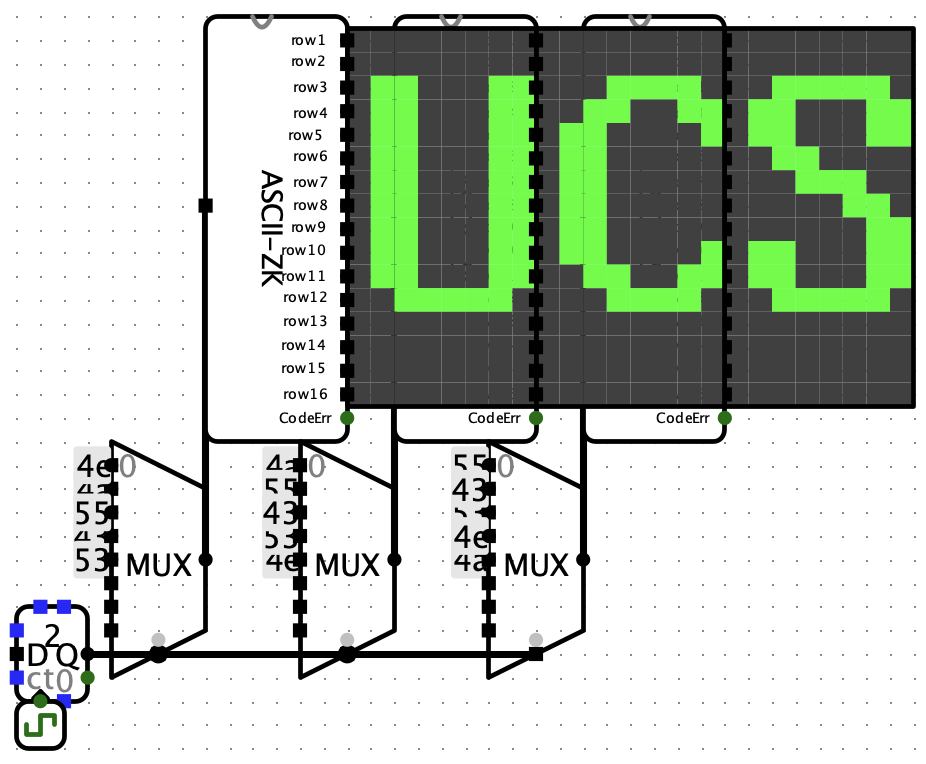
\includegraphics[width=0.4\textwidth]{assets/p1.1.png}}
    \subcaptionbox{}{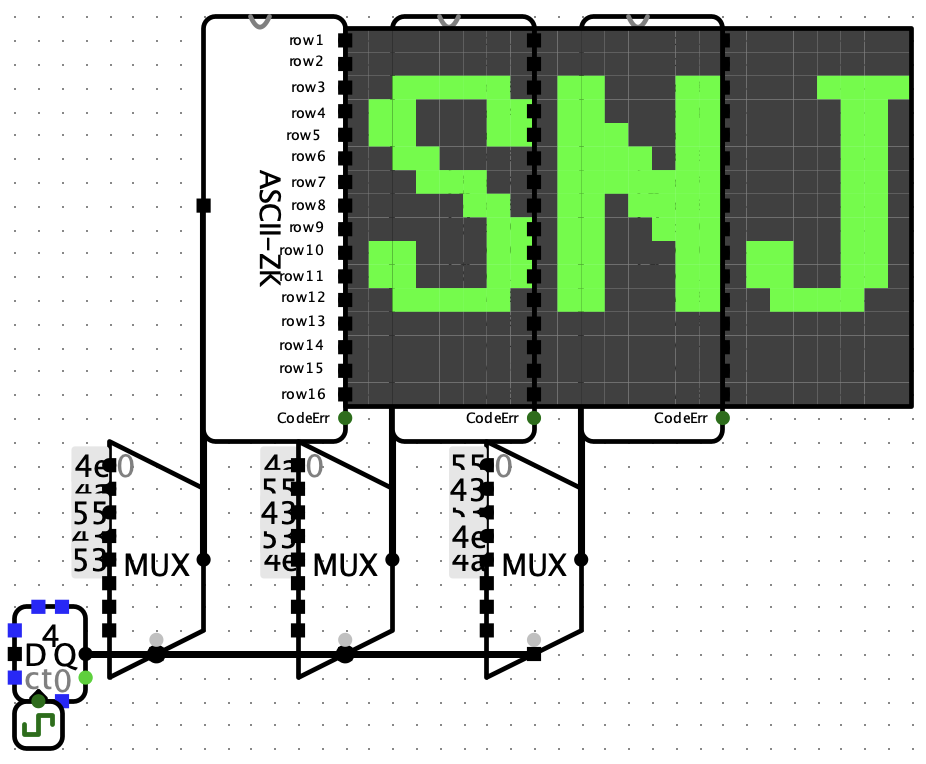
\includegraphics[width=0.4\textwidth]{assets/p1.2.png}}
    \caption{ROM 滚动显示器仿真结果}
\end{figure}

\subsection{时钟触发边沿不一致的影响}

可能导致数据读写错乱、时序违例与逻辑混乱，从而引发不可预期的行为，甚至系统崩溃。

\subsection{CPU 停机方法}

软件层面上，可在程序的末尾添加一条跳转到自身当前地址的无条件跳转指令，即
\texttt{loop: j loop}，使 CPU 进入死循环，从而达到停机的效果。

\end{document}
